\documentclass[10pt,conference,compsocconf]{IEEEtran}

\usepackage{hyperref}
\usepackage{graphicx}	% For figure environment
\usepackage{placeins}
\usepackage{float}


\begin{document}
\title{Machine Learning Project I}

\author{
  Andres Montero, Elias Poroma, Jonas J\"aggi\\
  \textit{School of Computer and Communication Sciences, EPFL, Switzerland}
}

\maketitle

\begin{abstract}
  Machine learning is a field of artificial intelligence that uses statistical 
  techniques to give computer systems the ability to "learn" from data, 
  without being explicitly programmed. And in this project it is applied 
  to estimate the likelihood that a given feature set is the result of a
  specific particle, for example the Higss Boson.
  This report gives an overview of six machine learning methods that were implemented
  and evaluated by the accuracy of their predictions. It describes 
  the pre-processing, data cleaning and algorithms used in order to find which
  model has the best fit for the data provided. After comparing these results,
  the machine learning method which reaches the highest accuracy is Least Squares.

\end{abstract}

\section{Introduction}

The Higgs boson is an elementary particle in the Standard Model of 
particle physics, produced by the quantum excitation of the Higgs field
and explains why some particles have mass~\cite{wiki01}. To confirm 
the existence of this particle, the CERN made several experiments from 
which the data is obtained and the objective of the here presented work is to present 
a machine learning model that will give the best prediction. However 
the data also contains measurements of other possible particles, so the main 
objective is to determine if the data of each experiment belongs to 
the higss boson or to the other particles depending on the values provided
on the data set. The training data set contains N=250000 measurements, and each measurement
is described by 30 features and one label, which is 's' correct positive
or 'b' false positive. Another 568.268 measurements with
the same 30 features and the corresponding labels are available for Kaggle~\cite{kaggle01} in order to evaluate the submissions.

\section{Data Pre-Processing}

\label{sec:Data Pre-Processing}

It is crucial that the data is understood and that the noise existing in the 
data is cleaned. First the models were trained without data pre-processing
and this lead to bad results. To avoid this and also to 
show the impact that data cleaning has on a machine learning model the different
steps of the process are described.

\subsection{Understanding the Data}
In the data presented there are 30 features, which are explained in 
the paper of the Higgs Challenge ~\cite{higgs_challenge01}. After a 
close analysis of this information, the results are:

\begin{itemize}
 \label{text:categorical}
\item The feature in column 22 \texttt{PRI\_jet\_num} is a categorical feature,
with discrete values of (0,1,2,3). For this reason it should be considered
for categorical extraction from the data.
\item Depending on the values of \texttt{PRI\_jet\_num}  we have other columns
where the value is undefined, therefore these columns should be dropped 
on each categorical training.
\item Some feature may have the value -999, which means that
independently of the category they belong to, they are
undefined too. This delivers
noise to the model, so we replace them with the mean of the column in each
case.
\item After that we need to remove the outliers values, as we are using models
depending on MSE which penalizes heavily the outliers values, We use IQR technique ~\cite{IQR01} to replace outliers.

\end{itemize}

\subsection{Polynomials, Standardization, Offset}
 \label{text:datasteps}
\begin{itemize}
\item Polynomials are used in the models because linear models may cause
underfiting, however the degree of the polynomials should be calibrated carefully
to avoid over-fitting.
\item Once the polynomials are ready it is needed to standardize the data 
as the models we used converge faster with this feature, for this purpose 
the values (mean, standard deviation) from the train data  are used.
\item Adding one vector of "ones" as the offset in the data set also know as the
"bias" term.

\end{itemize}
\section{Models-Machine Learning}
For this project we implemented 6 different models to make the predictions, 
and for each of them we implemented different data cleaning stages
to avoid noise in the model. Then to assure that the model will work as 
expected with new values, k-fold cross validation was used with a values of
k=5 to split the data in 5 even groups, where 4 groups are used for training 
and one group is used for test. 
The results found for the different six models are summarized in Table~\ref{tab:models}.
The best results were obtained with ``Least Squares'' model, so this will
be used to describe in detail how the results were obtained.
To begin with the training of our models first we analyzed different scenarios: 

\begin{enumerate}
\item Training the model - Standardization \\
First each model trained with the entire set of data, without applying categorical 
training. In this case is only applied standardization as explained in ~\ref{text:datasteps}
The results obtained for the accuracy is :  \texttt{0.774\%}
With these results we clearly deduct that more cleaning stages were necessary to understand
the data and achieve that our model behaves as expected.
\item Training the model - Removing Outliers \\
Analyzing the previous step, we realized that the model showed really high values, to fix
this problem we proceed with the removing outliers step explained in ~\ref{text:datasteps}.
The results obtained for the accuracy is :  \texttt{0.788\%}.\\
The results of the 6  models when applied the two steps mentioned before are summarized in 
the following table:
\end{enumerate}

\begin{table}[H]
  \caption{Machine Learning Models - Results.}
  \label{tab:models}
\begin{tabular}{|l|l|l|l|}
\hline
\textbf{Model}                                                              & \textbf{Accuracy} & \textbf{Hyper Param}                                      & \textbf{gamma, iterations} \\ \hline
\begin{tabular}[c]{@{}l@{}}Least Squeares\\   GD\end{tabular}               &    0.718        & \begin{tabular}[c]{@{}l@{}}degree=1\\ lambda=\end{tabular} & 0.01,          2500 \\ \hline
\begin{tabular}[c]{@{}l@{}}Least Squeares\\   SGD\end{tabular}              &     0.657         & \begin{tabular}[c]{@{}l@{}}degree=1\\ lambda=\end{tabular} & 0.0001, 2000         \\ \hline
Least Squeares                                                              &   0.774             & \begin{tabular}[c]{@{}l@{}}degree=2\\ lambda=-\end{tabular} & -          \\ \hline
\begin{tabular}[c]{@{}l@{}}Ridge\\   Regression\end{tabular}                &   0.773           & \begin{tabular}[c]{@{}l@{}}degree=2\\ lambda=5e-13\end{tabular} & -          \\ \hline
\begin{tabular}[c]{@{}l@{}}Logistic\\   Regression\end{tabular}             & 0.731           & \begin{tabular}[c]{@{}l@{}}degree=1\\ lambda=\end{tabular} & 0.1, 2500          \\ \hline
\begin{tabular}[c]{@{}l@{}}Regularized\\   Logistic Regression\end{tabular} & 0.731             & \begin{tabular}[c]{@{}l@{}}degree=1\\ lambda =150\end{tabular} & 0.1, 2500       \\ \hline
\end{tabular}
\end{table}
 
 Finally to obtain the official result presented to kaggle the model will also be trained depending
 on the categorical values as explained in~\ref{text:categorical}. The result obtained for the 
 accuracy is :  \texttt{0.8078\%}.\\

After the data cleaning stage is completed the weights are initialized as a column 
of ones, then we define that all the data processing functions are true, as 
discussed before gives a better result. Then we input the value for the selected 
model and define the maximum iterations and start the cross validation step 
to assure that the models will work as expected. Once this is completed a grid search
method is applied for the degree of the polynomials and also for the best
lambda used to penalize the model and avoid over-fitting in case that the 
degree found in the grid search is to high. The result shows that the best degree
is 2  and the best lambda is 5e-13 as you can see in the figures ~\ref{fig:best_degree}. 
With these results it is deduced that the lambda value is almost zero
which could cause that the model over-fits if the degree of the polynomial was
higher, however with just a value of two in the degree, the risk of over-fitting is
low, therefore the lambda value will be omitted. 
Once the best hyper-parameters are found the model can start with the training
for each of the categorical values, giving a prediction to each categorical value
and appending this to final result that will be saved as an excel file.

\begin{figure}[H]
  \centering
  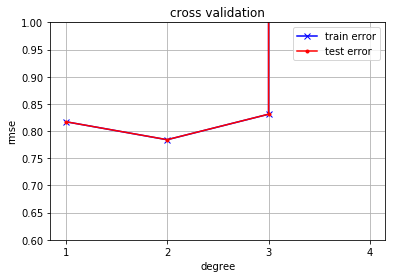
\includegraphics[width=\columnwidth]{cross_validation_degree}
  \caption{RMSE for different degrees of polynomial expansion - Ridge regression.}
  \vspace{-3mm}
  \label{fig:best_degree}
\end{figure}


\begin{figure}[H]
  \centering
  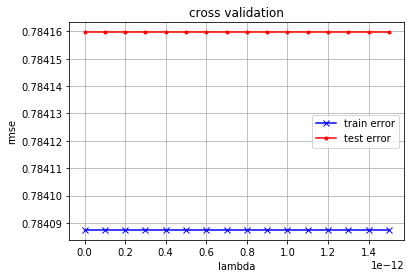
\includegraphics[width=\columnwidth]{cross_validation_lambda}
  \caption{RMSE for different regularization values - Ridge regression}
  \vspace{-3mm}
  \label{fig:best_lambda}
\end{figure}



\section{Results and Summary}
To predict if the data of each row corresponds to the Higss boson
6 different models are proposed, which are trained with k-fold cross validation
method and grid search to find the best hyper-parameters. 
Different data pre processing stages are applied to evaluate the best results. 
\textbf{Least Squares} has the best behavior for the data provided and 
the highest accuracy (\textbf{0.80780} KAGGLE) .
A detailed explanation of how to run the program is
in the ``read me'' file presented with the results.


\bibliographystyle{IEEEtran}
\bibliography{literature}

\end{document}
